\documentclass[portrait,final,archD,fontscale=0.477]{baposter}
% Currently set to 24" wide by 36" tall (archD).
% See baposter.cls for info on changing paper dimensions

\usepackage{calc}
\usepackage{graphicx}
\usepackage{amsmath}
\usepackage{amssymb}
\usepackage{relsize}
\usepackage{multirow}
\usepackage{rotating}
\usepackage{bm}
\usepackage{url}
\usepackage{color}

\usepackage{graphicx}
\usepackage{multicol}

%\usepackage{times}
%\usepackage{helvet}
%\usepackage{bookman}
\usepackage{palatino}

\newcommand{\captionfont}{\footnotesize}

%%%%%%%%%%%%%%%%%%%%%%%%%%%%%%%%%%%%%%%%%%%%%%%%%%%%%%%%%%%%%%%%%%%%%%%%%%%%%%%%
%%%% Some math symbols used in the text
%%%%%%%%%%%%%%%%%%%%%%%%%%%%%%%%%%%%%%%%%%%%%%%%%%%%%%%%%%%%%%%%%%%%%%%%%%%%%%%%

%%%%%%%%%%%%%%%%%%%%%%%%%%%%%%%%%%%%%%%%%%%%%%%%%%%%%%%%%%%%%%%%%%%%%%%%%%%%%%%%
% Multicol Settings
%%%%%%%%%%%%%%%%%%%%%%%%%%%%%%%%%%%%%%%%%%%%%%%%%%%%%%%%%%%%%%%%%%%%%%%%%%%%%%%%
\setlength{\columnsep}{1.5em}
\setlength{\columnseprule}{0mm}

%%%%%%%%%%%%%%%%%%%%%%%%%%%%%%%%%%%%%%%%%%%%%%%%%%%%%%%%%%%%%%%%%%%%%%%%%%%%%%%%
% Save space in lists. Use this after the opening of the list
%%%%%%%%%%%%%%%%%%%%%%%%%%%%%%%%%%%%%%%%%%%%%%%%%%%%%%%%%%%%%%%%%%%%%%%%%%%%%%%%
\newcommand{\compresslist}{%
\setlength{\itemsep}{1pt}%
\setlength{\parskip}{0pt}%
\setlength{\parsep}{0pt}%
}

%%%%%%%%%%%%%%%%%%%%%%%%%%%%%%%%%%%%%%%%%%%%%%%%%%%%%%%%%%%%%%%%%%%%%%%%%%%%%%
%%% Begin of Document
%%%%%%%%%%%%%%%%%%%%%%%%%%%%%%%%%%%%%%%%%%%%%%%%%%%%%%%%%%%%%%%%%%%%%%%%%%%%%%

\begin{document}

%%%%%%%%%%%%%%%%%%%%%%%%%%%%%%%%%%%%%%%%%%%%%%%%%%%%%%%%%%%%%%%%%%%%%%%%%%%%%%
%%% Here starts the poster
%%%---------------------------------------------------------------------------
%%% Format it to your taste with the options
%%%%%%%%%%%%%%%%%%%%%%%%%%%%%%%%%%%%%%%%%%%%%%%%%%%%%%%%%%%%%%%%%%%%%%%%%%%%%%
% Define some colors

\definecolor{stevensred}{rgb}{0.6392,0.149,0.2196}
\definecolor{stevensgray}{rgb}{0.60392, 0.596, 0.60392}
\definecolor{airforceblue}{rgb}{0.36, 0.54, 0.66}

%%
\begin{poster}%
  % Poster Options
  {
  % Show grid to help with alignment
  grid=false,
  % Column spacing
  colspacing=1em,
  % Color style
  bgColorOne=white,
  bgColorTwo=white,
  borderColor=airforceblue,
  headerColorOne=blue,
  headerColorTwo=blue,
  headerFontColor=airforceblue,
  boxColorOne=white,
  boxColorTwo=white,
  % Format of textbox
  textborder=rectangle,
  % Format of text header
  eyecatcher=true,
  headerborder=closed,
  headerheight=0.1\textheight,
%  textfont=\sc, An example of changing the text font
  headershape=rectangle,
  headershade=shadelr,
  headerfont=\Large\bf\textsc, %Sans Serif
  textfont={\setlength{\parindent}{1.5em}},
  boxshade=plain,
%  background=shade-tb,
  background=plain,
  linewidth=2pt
  }
  % Eye Catcher
  {\begin{minipage}{8em}
   \hfill\vspace{1in}
  \end{minipage} } % Empty space, replace with image if desired
  % Title
  {\bf \textsc{  Bayesian Learning with Generalized Kernels for Occupancy Map Prediction} }
  % Authors
  {\textsc{  Kevin Doherty, Jinkun Wang, and Brendan Englot \\ Stevens Institute of Technology, Hoboken NJ}}
  % University logo
  {% The makebox allows the title to flow into the logo, this is a hack because of the L shaped logo.
    
\includegraphics[height=9.0em]{img/stevenslogo}
  }

%%%%%%%%%%%%%%%%%%%%%%%%%%%%%%%%%%%%%%%%%%%%%%%%%%%%%%%%%%%%%%%%%%%%%%%%%%%%%%
%%% Now define the boxes that make up the poster
%%%---------------------------------------------------------------------------
%%% Each box has a name and can be placed absolutely or relatively.
%%% The only inconvenience is that you can only specify a relative position 
%%% towards an already declared box. So if you have a box attached to the 
%%% bottom, one to the top and a third one which should be in between, you 
%%% have to specify the top and bottom boxes before you specify the middle 
%%% box.
%%%%%%%%%%%%%%%%%%%%%%%%%%%%%%%%%%%%%%%%%%%%%%%%%%%%%%%%%%%%%%%%%%%%%%%%%%%%%%
    %
    % A coloured circle useful as a bullet with an adjustably strong filling
    \newcommand{\colouredcircle}{%
      \tikz{\useasboundingbox (-0.2em,-0.32em) rectangle(0.2em,0.32em); \draw[draw=black,fill=lightblue,line width=0.03em] (0,0) circle(0.18em);}}

%%%%%%%%%%%%%%%%%%%%%%%%%%%%%%%%%%%%%%%%%%%%%%%%%%%%%%%%%%%%%%%%%%%%%%%%%%%%%%
  \headerbox{Introduction}{name=problem,column=0,row=0}{
%%%%%%%%%%%%%%%%%%%%%%%%%%%%%%%%%%%%%%%%%%%%%%%%%%%%%%%%%%%%%%%%%%%%%%%%%%%%%%

Maps express rich environmental information necessary for autonomous robots to avoid collision and make planning and navigation decisions. Current sensors used in robot perception are limited by noise and sparsity. We propose a novel algorithm leveraging recent advances in data structures for mapping, sparse kernels, and Bayesian nonparametric inference to perform mapping with sparse and noisy range-sensors. The resulting inference model has several desirable properties in comparison to existing methods, including speed of computation, the ability to be recursively updated without approximation, and consistency between batch and online inference.

}

%%%%%%%%%%%%%%%%%%%%%%%%%%%%%%%%%%%%%%%%%%%%%%%%%%%%%%%%%%%%%%%%%%%%%%%%%%%%%%
  \headerbox{References}{name=references,column=0,above=bottom}{
%%%%%%%%%%%%%%%%%%%%%%%%%%%%%%%%%%%%%%%%%%%%%%%%%%%%%%%%%%%%%%%%%%%%%%%%%%%%%%
    \smaller
    \bibliographystyle{ieee}
    \renewcommand{\section}[2]{\vskip 0.05em}
      \begin{thebibliography}{1}\itemsep=-0.01em
      \setlength{\baselineskip}{0.4em}
\bibitem{vegabrown} W.R. Vega-Brown, M. Doniec, and N.G. Roy, "Nonparametric Bayesian inference on multivariate exponential families," \textit{Advances in Neural Information Processing Systems}, pp. 2546-2554, 2014.

\bibitem{sparsekernel} A. Melkumyan and F. Ramos, "A Sparse Covariance Function for Exact Gaussian Process Inference in Large Datasets," \textit{Proceedings of the International Joint Conferences on Artificial Intelligence Organization}, vol. 9, pp. 1936-1942, 2009.

\bibitem{jwang} J. Wang and B. Englot, "Fast, Accurate Gaussian Process Occupancy Maps via Test-Data Octrees and Nested Bayesian Fusion," \textit{Proceedings of the IEEE International Conference on Robotics and Automation}, pp. 1003-1010, May 2016.

      \end{thebibliography}
   \vspace{0.05em}
  }

%%%%%%%%%%%%%%%%%%%%%%%%%%%%%%%%%%%%%%%%%%%%%%%%%%%%%%%%%%%%%%%%%%%%%%%%%%%%%%
  \headerbox{Bayesian Inference Model}{name=method,column=0,below=problem, above=references}{
%%%%%%%%%%%%%%%%%%%%%%%%%%%%%%%%%%%%%%%%%%%%%%%%%%%%%%%%%%%%%%%%%%%%%%%%%%%%%%

We abbreviate the probability that a map cell $m$ is occupied $p(m=1|x_*)$ as $p(m|x_*)$. As in standard occupancy grid mapping, the cell $m$ is occupied with probability $p(m|x_*)$ and free with probability $1-p(m|x_*)$. That is, $m \sim \mathit{Ber}(\theta)$, with parameter $\theta = p(m | x_*)$. We seek to estimate the parameter $\theta$. To do so, we use the  nonparametric Bayesian inference model for exponential families in \cite{vegabrown}. With $\theta \sim \mathit{Beta}(\alpha, \beta)$, the predicted mean and variance of $\theta$ are as follows:
\begin{align}
	\mathbf{E}[\theta] = \frac{\alpha}{\alpha + \beta}
\end{align}
\begin{align}
	\mathbf{Var}[\theta] = \frac{\alpha \beta}{(\alpha + \beta)^2 (\alpha + \beta + 1)}
\end{align}
where $\alpha$ and $\beta$ are hyperparameters. At each time step we can apply exact recursive updates to the hyperparameters
\begin{align}
	\alpha_t &= \alpha_{t-1} + \bar{y} \label{eq:update-a}\\
	\beta_t &= \beta_{t-1} + \bar{k} - \bar{y} \label{eq:update-b}
\end{align}
in which $\bar{k}$ and $\bar{y}$ are the results of the following kernel computations:
\begin{align}
	\bar{y} &= \sum_{i=1}^N k(x_i, x_*)y_i \\
	\bar{k} &= \sum_{i=1}^N k(x_i, x_*). 
\end{align}

The quantities $\alpha_0$ and $\beta_0$ represent prior pseudo-counts of the positive (occupied) and negative (free) classes respectively.

We also take advantage of variance predictions in a similar fashion to previous work \cite{jwang}. We use the following model of state for cells in the environment
\begin{align}
	\text{state} = \begin{cases} \text{free,} & \text{if }p < p_{free}, \sigma^2 < \sigma^2_{th} \\
	\text{occupied,} & \text{if } p > p_{occ}, \sigma^2 < \sigma^2_{th} \\
	\text{unknown,} & \text{otherwise} \end{cases}
\end{align}
where $p = \mathbf{E}[\theta]$, and quantities $p_{free}$ and $p_{occ}$ are thresholds on the occupancy probability of cells deemed "free," and "occupied," respectively. The variance $\sigma^2$, is $\mathbf{Var}[\theta]$, which is thresholded by $\sigma^2_{th}$ to filter out predictions with high variance as "unknown."

We opt to use the sparse kernel presented in \cite{sparsekernel} to enable exact updates in equations \ref{eq:update-a} and \ref{eq:update-b}.
\begin{multline}
    k(x,x') = \\ \begin{cases}
        \sigma_0\big[\frac{2 + \cos(2\pi\frac{d}{l})}{3}(1 - \frac{d}{l}) + \frac{1}{2\pi}\sin(2\pi\frac{d}{l})\big] & \text{if } d < l\\
        0 & \text{if } d\geq l\\ \label{eq:sparse-kern}
        \end{cases}
\end{multline}
where $\sigma_0 > 0$ is a constant parameter of the kernel, $l > 0$ is the scale, and $d$ is the distance between $x$ and $x'$. 
}

%%%%%%%%%%%%%%%%%%%%%%%%%%%%%%%%%%%%%%%%%%%%%%%%%%%%%%%%%%%%%%%%%%%%%%%%%%%%%%
\headerbox{Test Data Octrees}{name=results,column=1,span=2,row=0}{
%%%%%%%%%%%%%%%%%%%%%%%%%%%%%%%%%%%%%%%%%%%%%%%%%%%%%%%%%%%%%%%%%%%%%%%%%%%%%%

\begin{multicols}{2}

To the right we show the core data structure involved in our approach to occupancy maps: the "test data octree" from \cite{jwang}, which allows us to prune our environment representation to a lower resolution.
\newline

\textbf{Top-left}: Standard occupancy grid mapping. \\

\textbf{Top-right}: Setup for prediction of the occupancy probability of all cells in block $3$. The extended block consists of all blocks within distance $l$ of block $3$ that contain sensor data or sampled free-space points. \\

\textbf{Bottom-left}: For each block, the data from the corresponding extended block is aggregated and inference is performed. \\

\textbf{Bottom-right}: Neighboring cells within a block with the same occupancy state are pruned.

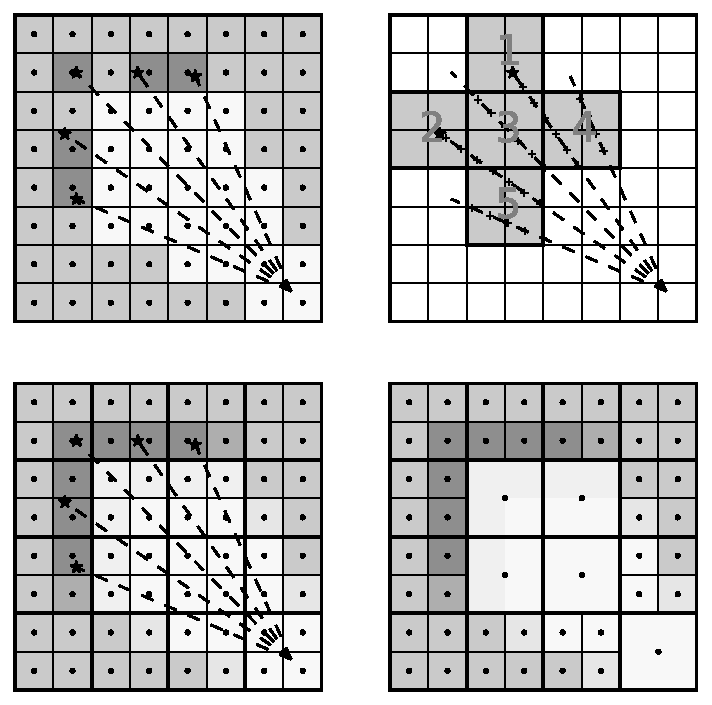
\includegraphics[width=0.9\linewidth]{img/grid_octrees_predict}

\end{multicols}

}

%%%%%%%%%%%%%%%%%%%%%%%%%%%%%%%%%%%%%%%%%%%%%%%%%%%%%%%%%%%%%%%%%%%%%%%%%%%%%%
  \headerbox{Experimental Results}{name=background model,column=1, span=2,below=results, above=bottom}{
%%%%%%%%%%%%%%%%%%%%%%%%%%%%%%%%%%%%%%%%%%%%%%%%%%%%%%%%%%%%%%%%%%%%%%%%%%%%%%

{ 
	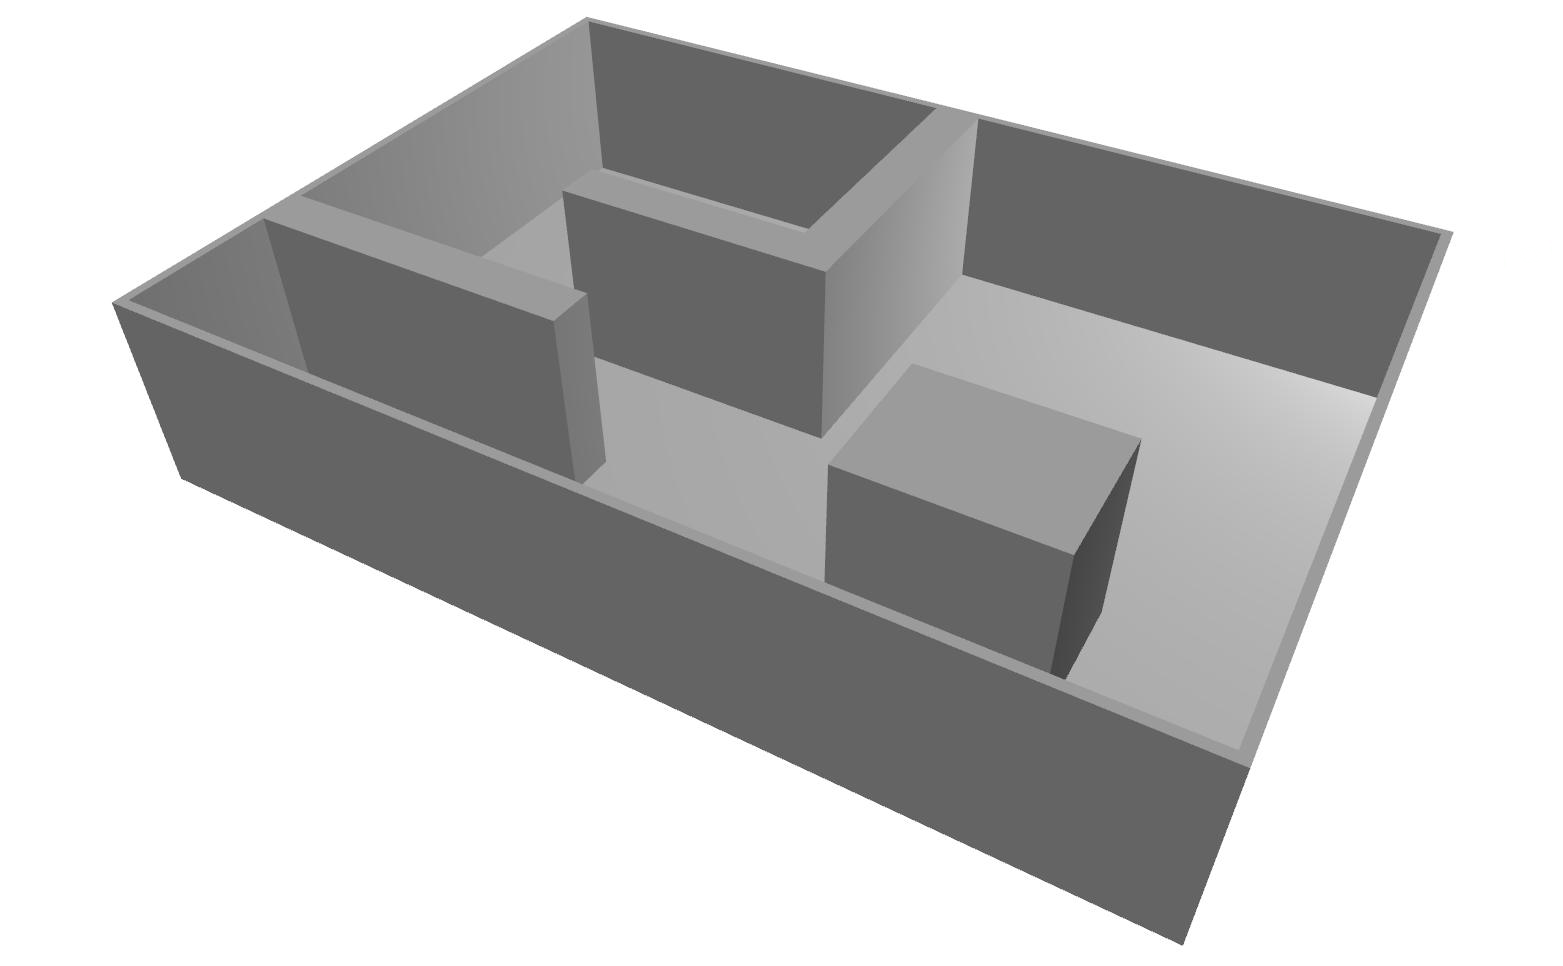
\includegraphics[width=0.23\linewidth]{img/sim_structured}
	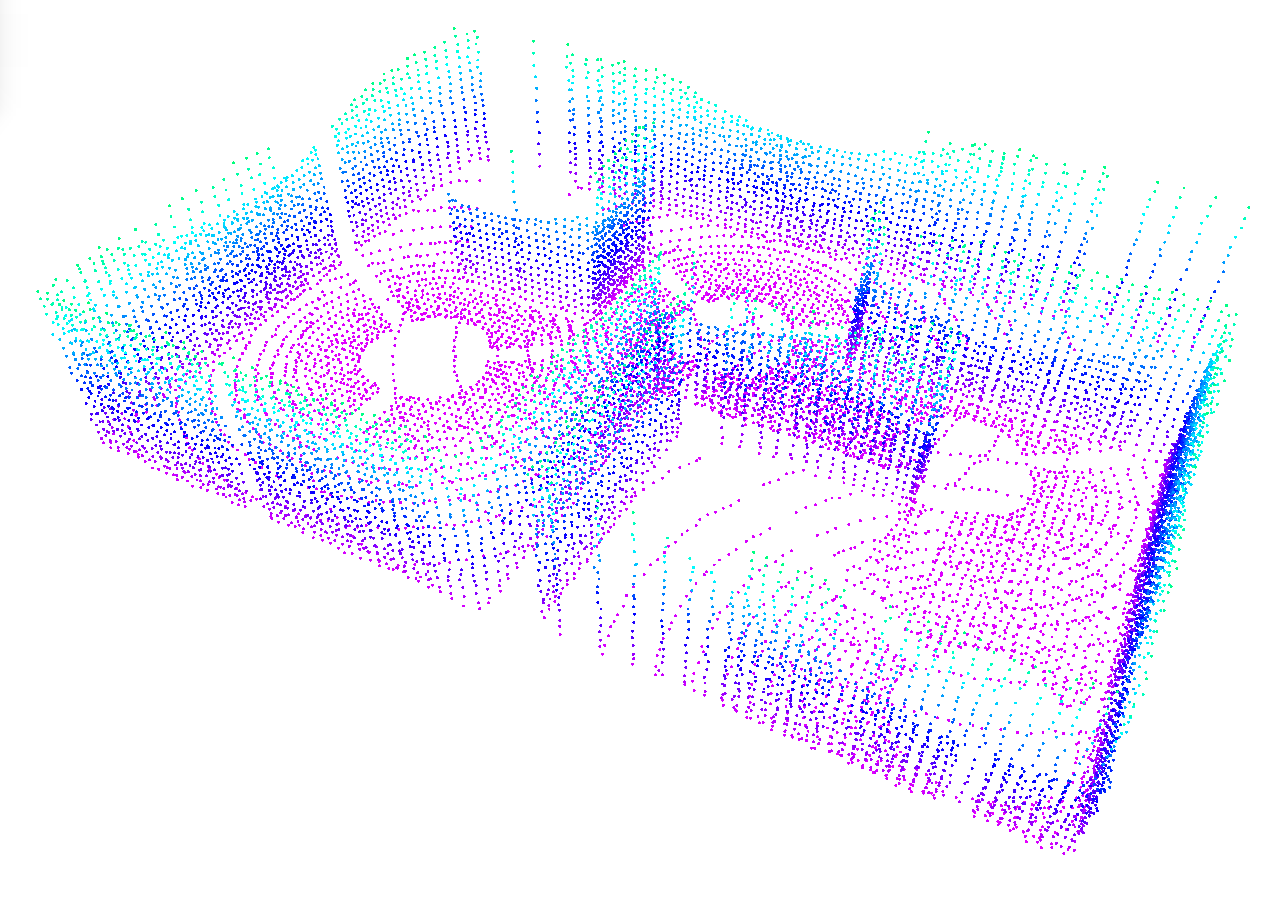
\includegraphics[width=0.23\linewidth]{img/sim_structured_raw}
	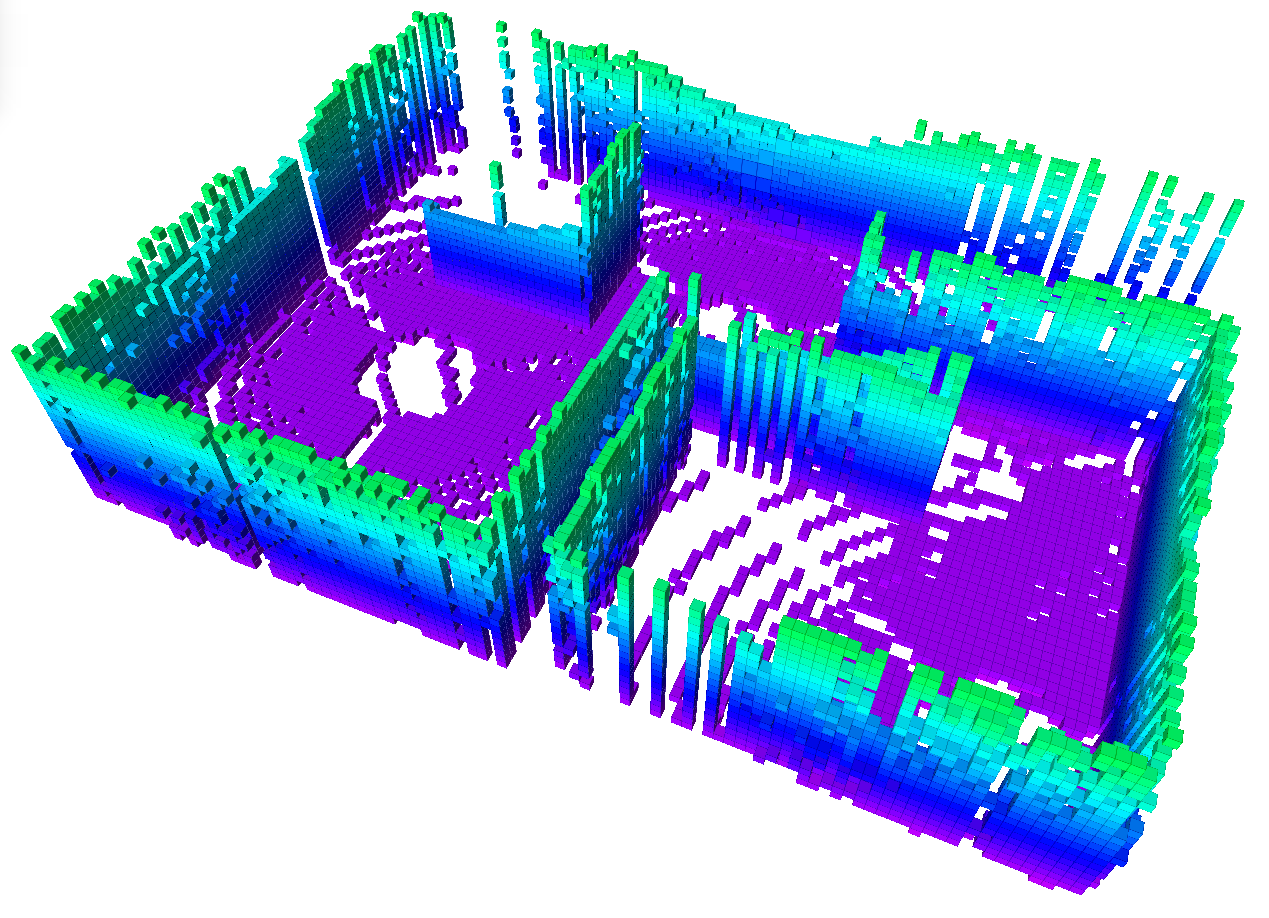
\includegraphics[width=0.23\linewidth]{img/sim_structured_octomap}
	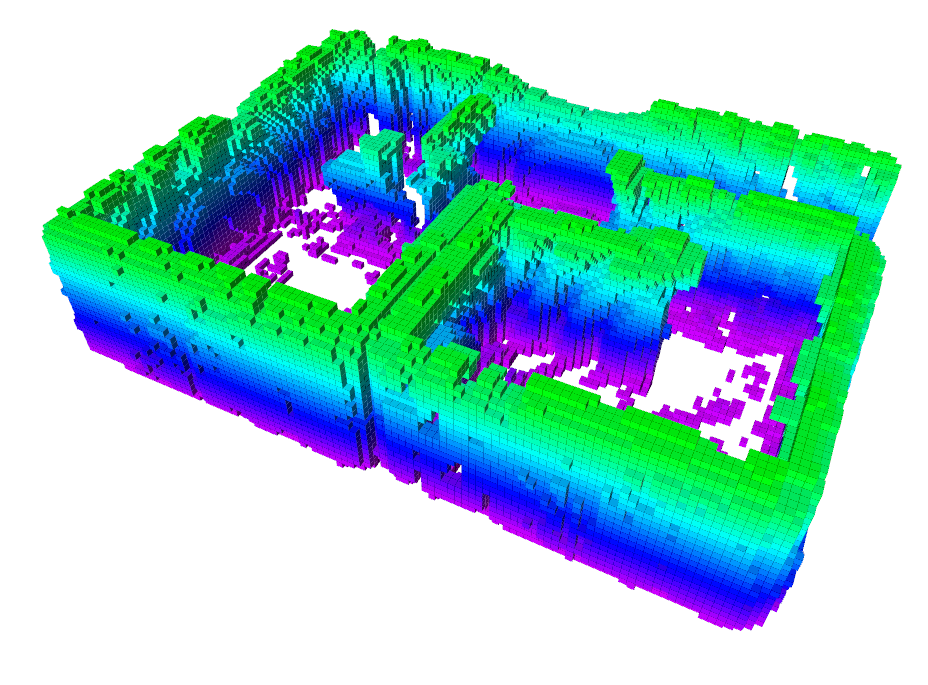
\includegraphics[width=0.23\linewidth]{img/sim_structured_bgk}
	
	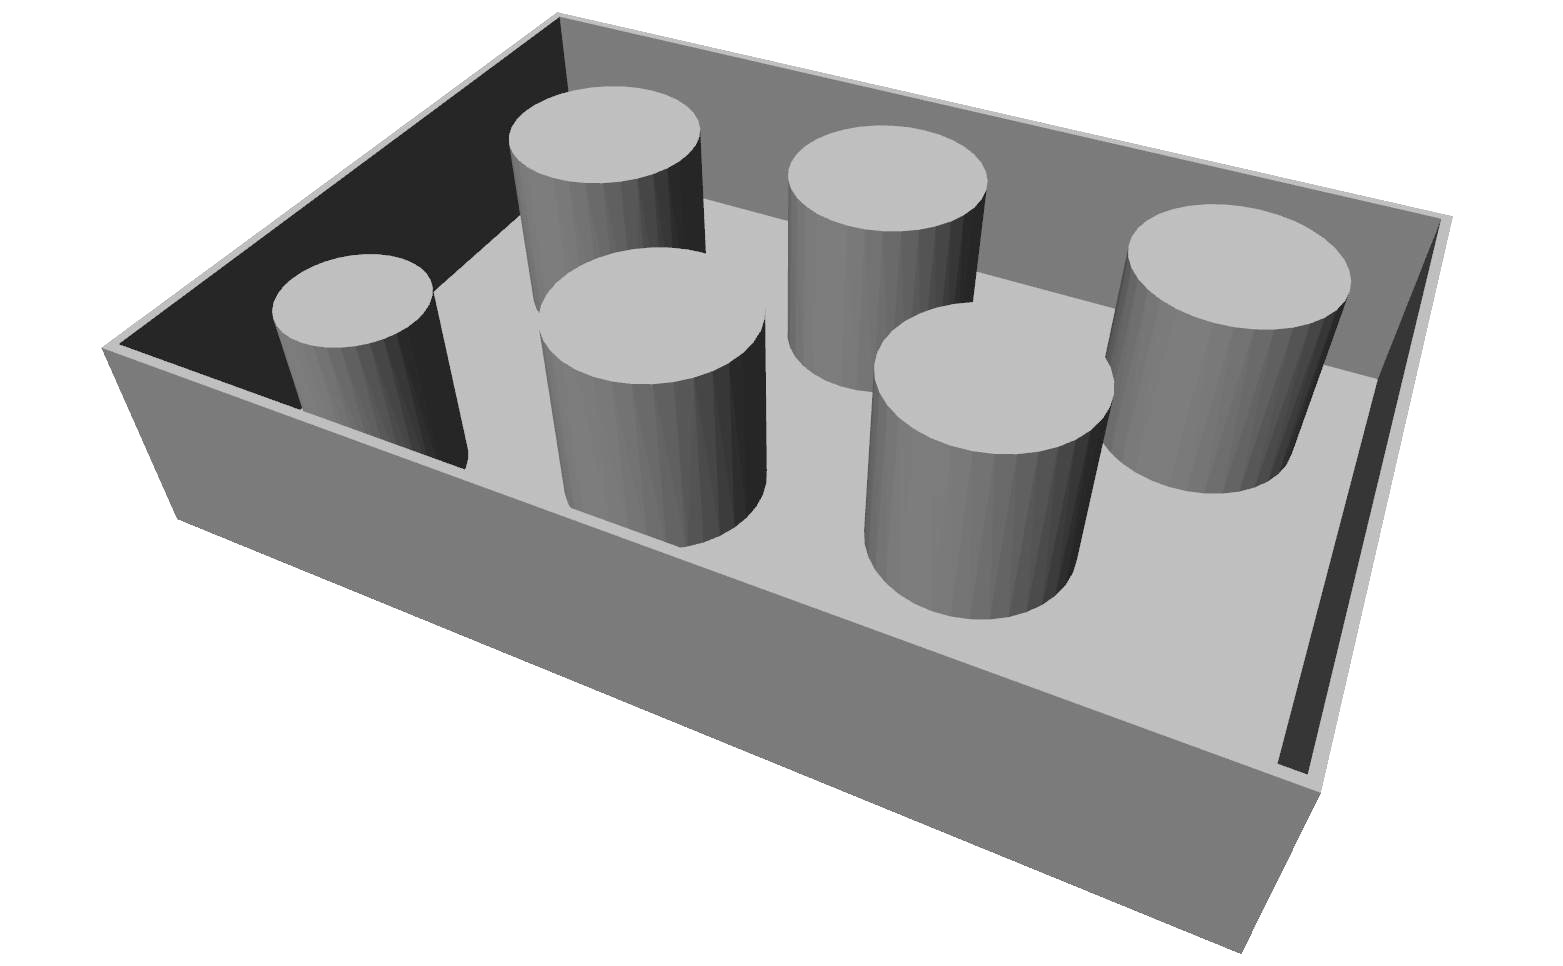
\includegraphics[width=0.23\linewidth]{img/sim_unstructured}
	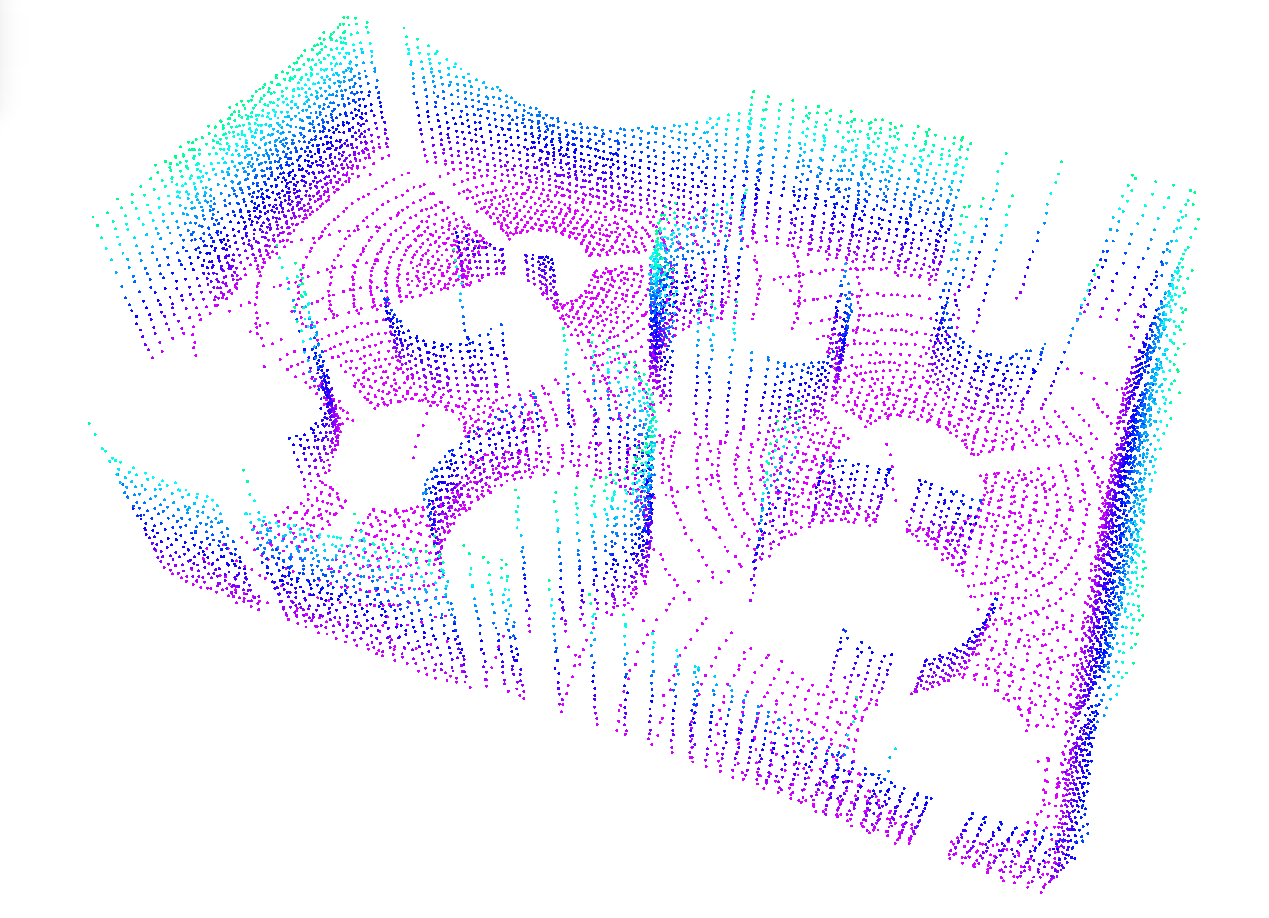
\includegraphics[width=0.23\linewidth]{img/sim_unstructured_raw}
	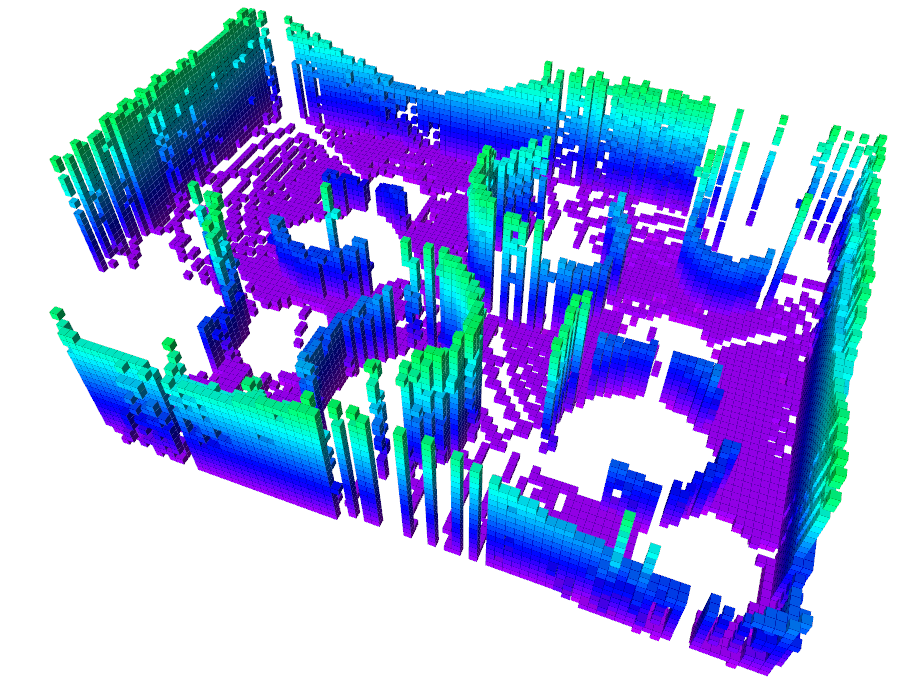
\includegraphics[width=0.23\linewidth]{img/octomap_sim_unstructured}
	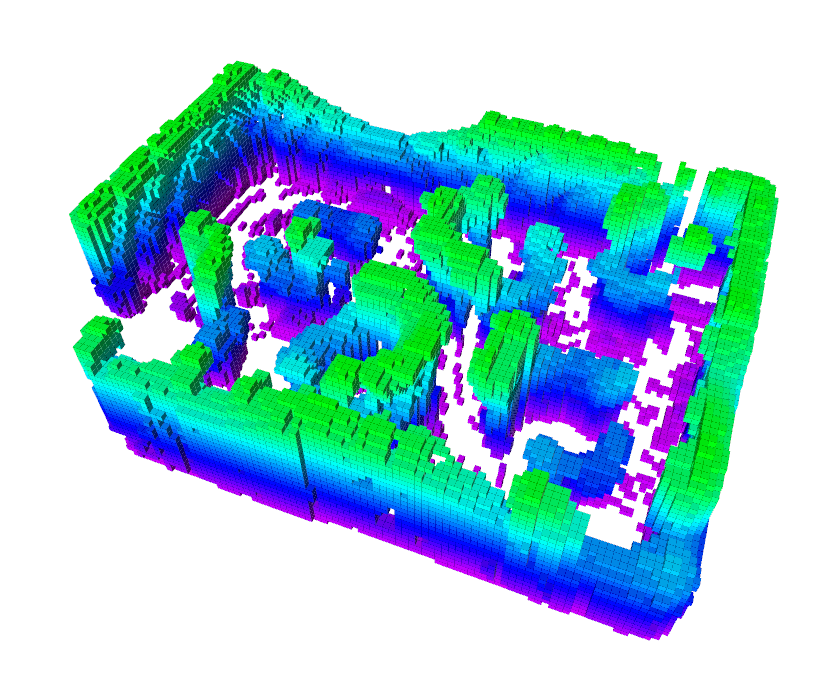
\includegraphics[width=0.23\linewidth]{img/sim_unstructured_bgk}
}
\\

We tested our method "Bayesian Generalized Kernel OctoMap" (BGKOctoMap) in simulated \textit{structured} (\textbf{top}) and \textit{unstructured} (\textbf{bottom}) environments. We show (colored by height), from \textbf{left} to \textbf{right}: 

\textbf{1)} The Gazebo simulation model for the environment

\textbf{2)} The simulated raw sensor data

\textbf{3)} The map produced by standard OctoMap

\textbf{4)} The result of applying our proposed method, BGKOctoMap.

\vspace{0.1em}

{
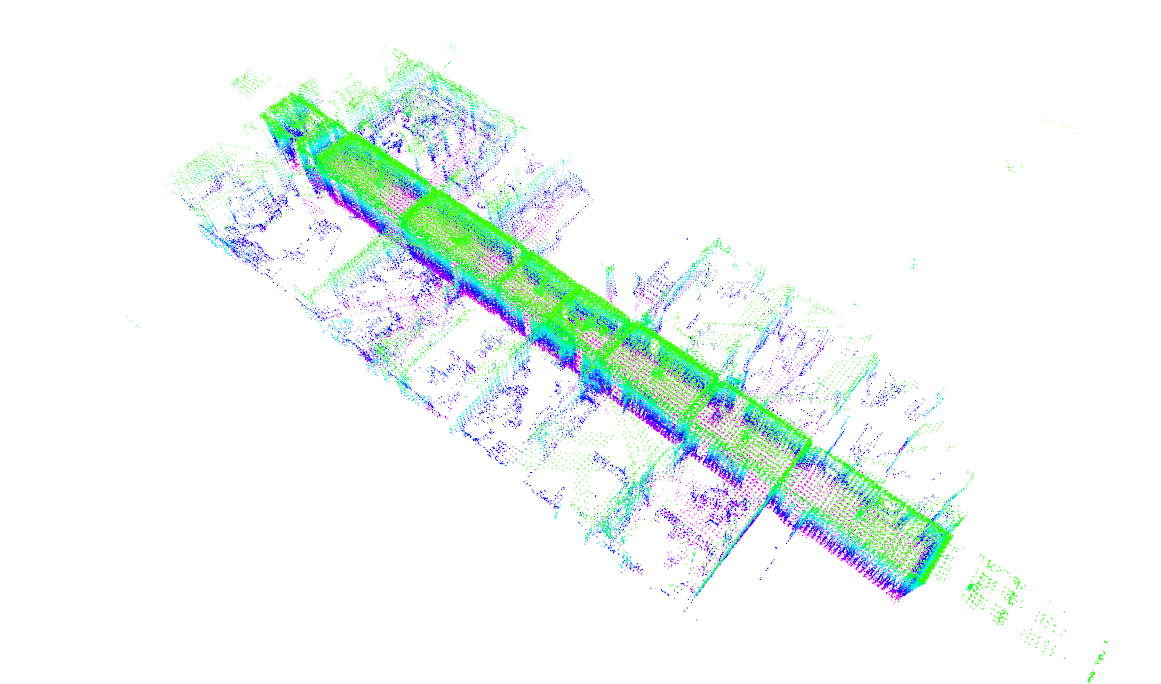
\includegraphics[width=0.3\linewidth]{img/fr_corridor_raw}
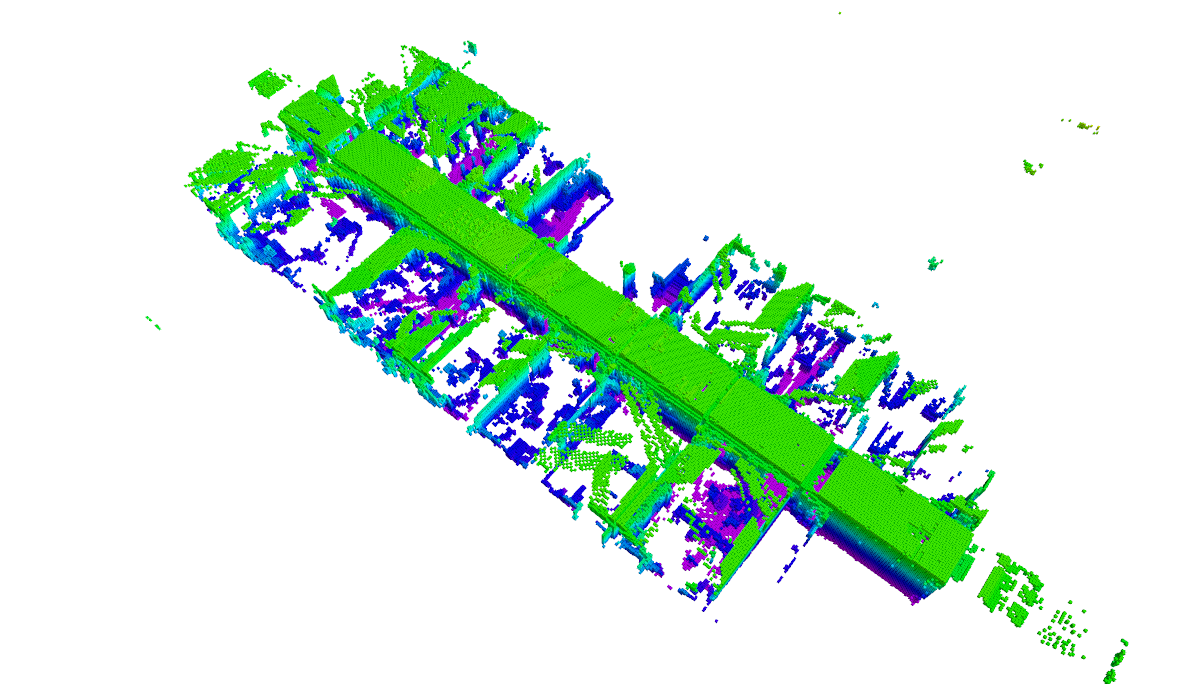
\includegraphics[width=0.3\linewidth]{img/fr_corridor_octomap}
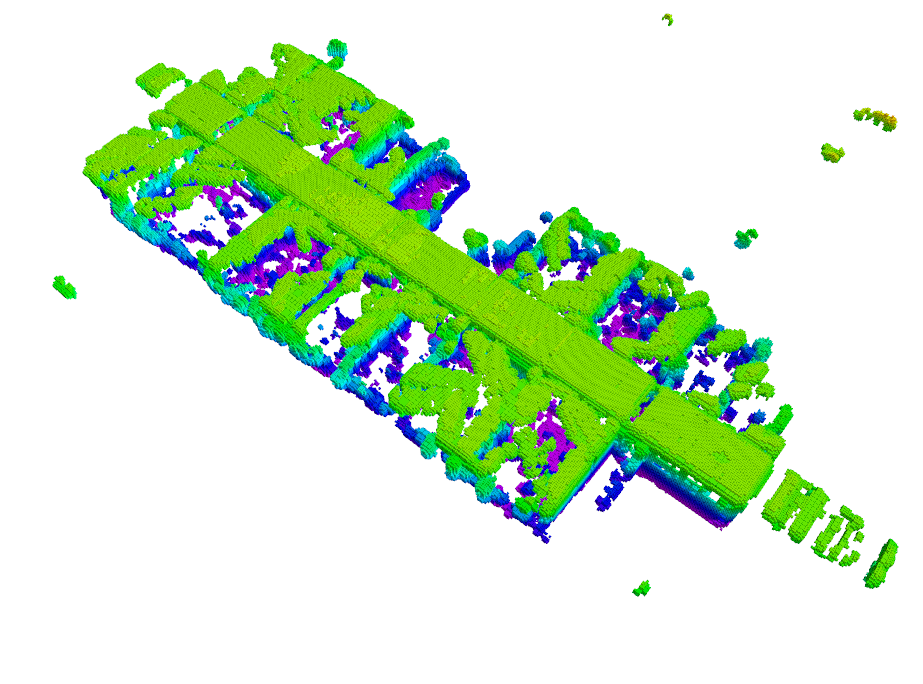
\includegraphics[width=0.3\linewidth]{img/fr_corri2}
}
\\

We also evaluated our method qualitatively on real data from the University of Freiburg, shown above. From \textbf{left} to \textbf{right} we have:

\textbf{1)} The raw range-sensor data from University of Freiburg Corridor FR-079

\textbf{2)} The map produced by standard OctoMap

\textbf{3)} The map produced by BGKOctoMap

\vspace{0.1em}
\begin{multicols}{2}

\hfill \\

{ 
	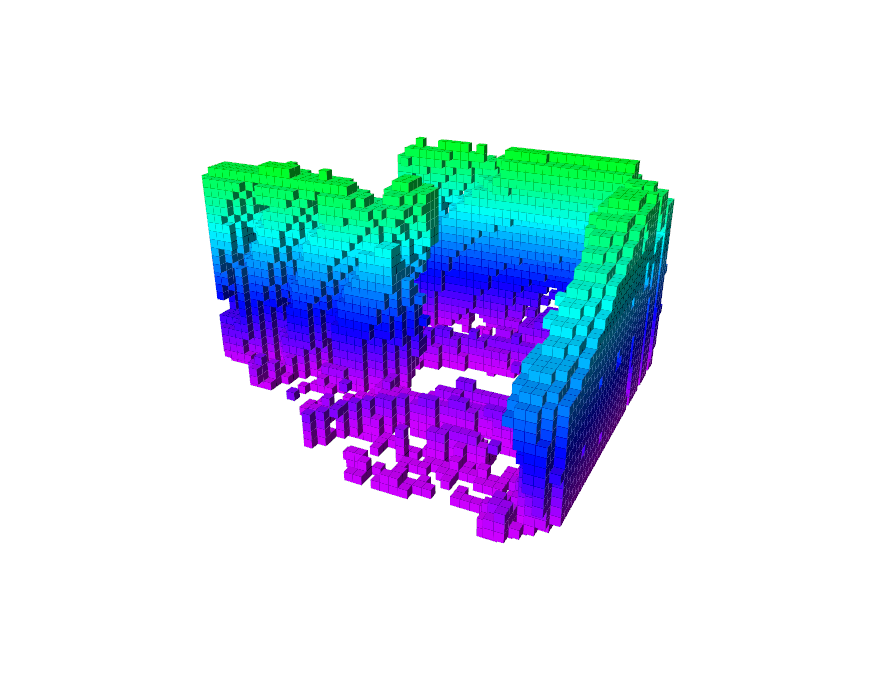
\includegraphics[width=0.23\linewidth]{img/long_term_gbk_1}
	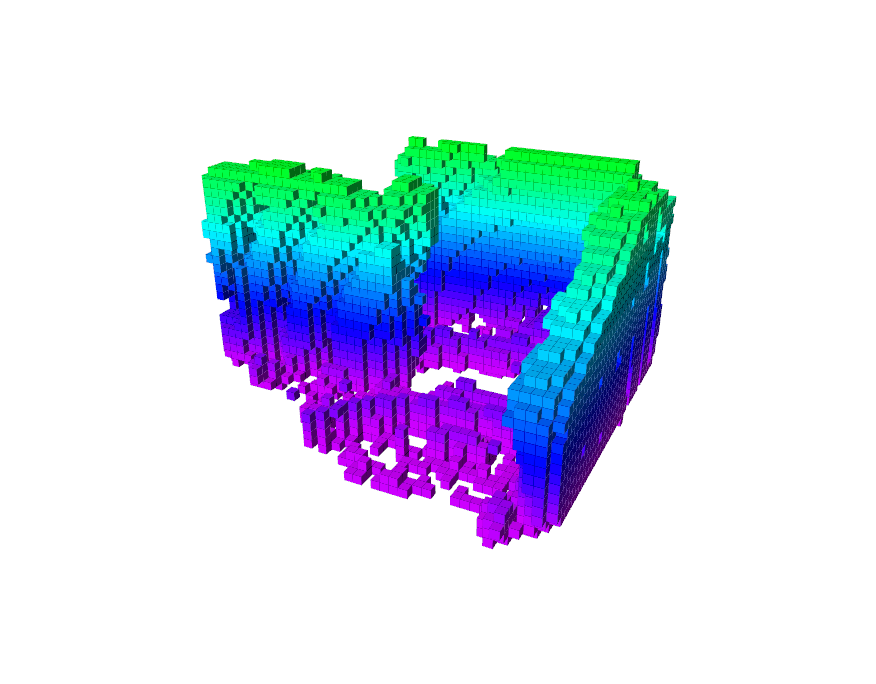
\includegraphics[width=0.23\linewidth]{img/long_term_gbk_15}
	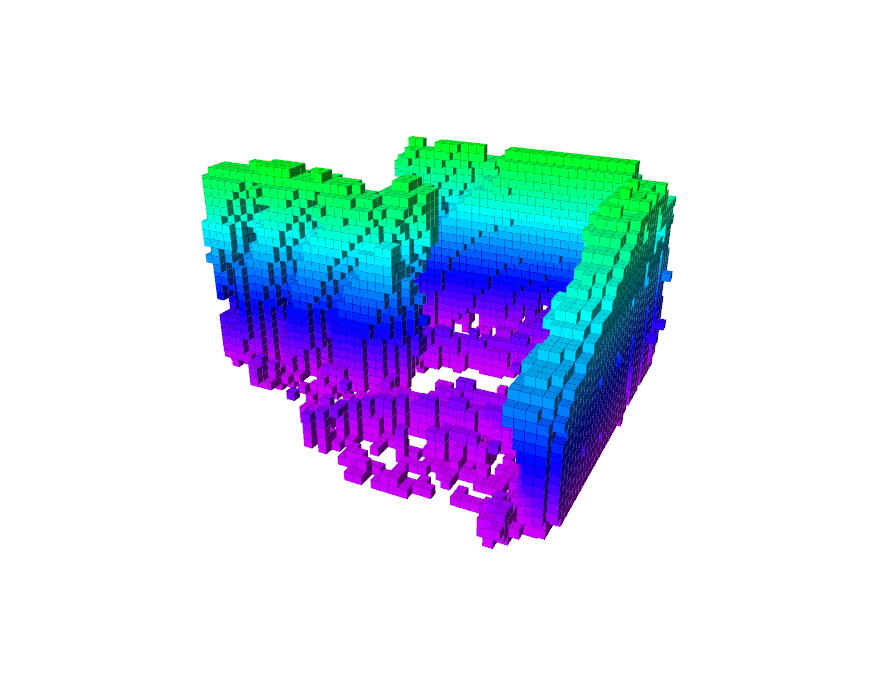
\includegraphics[width=0.23\linewidth]{img/long_term_gbk_30}
	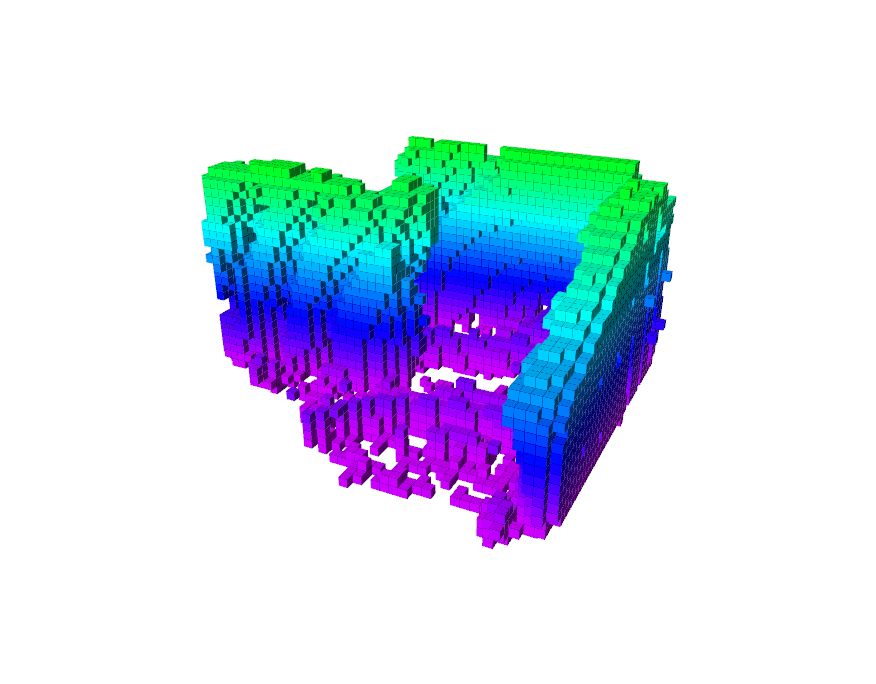
\includegraphics[width=0.23\linewidth]{img/long_term_gbk_60}
	}
	
	{
	
	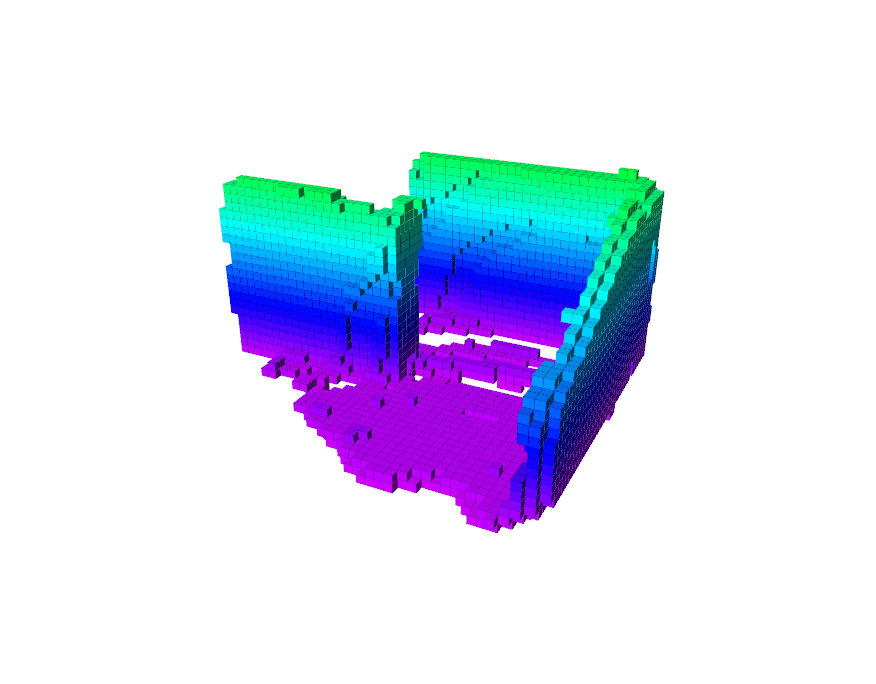
\includegraphics[width=0.23\linewidth]{img/long_term_gpoctomap_1}
	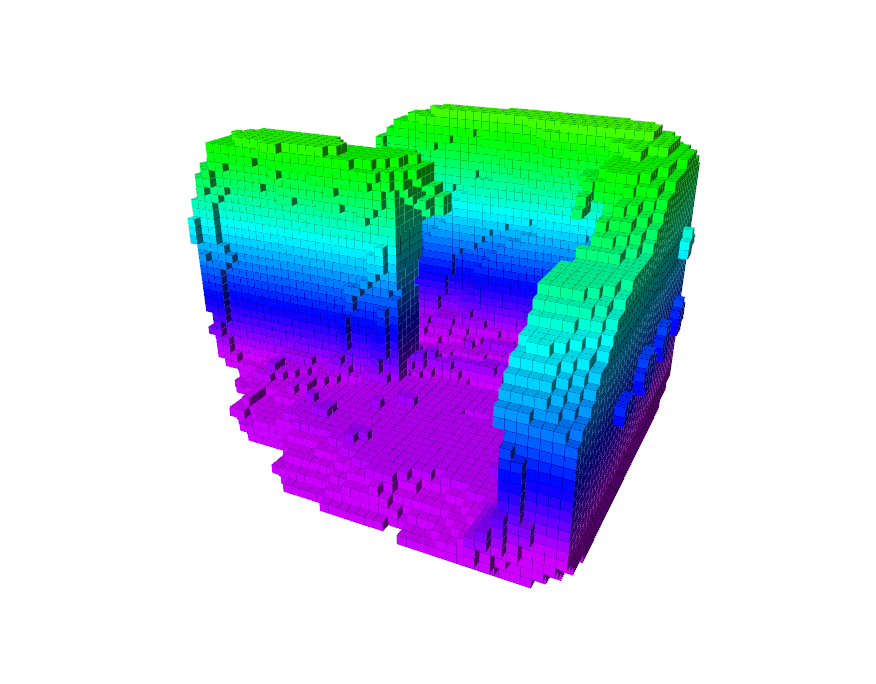
\includegraphics[width=0.23\linewidth]{img/long_term_gpoctomap_15}
	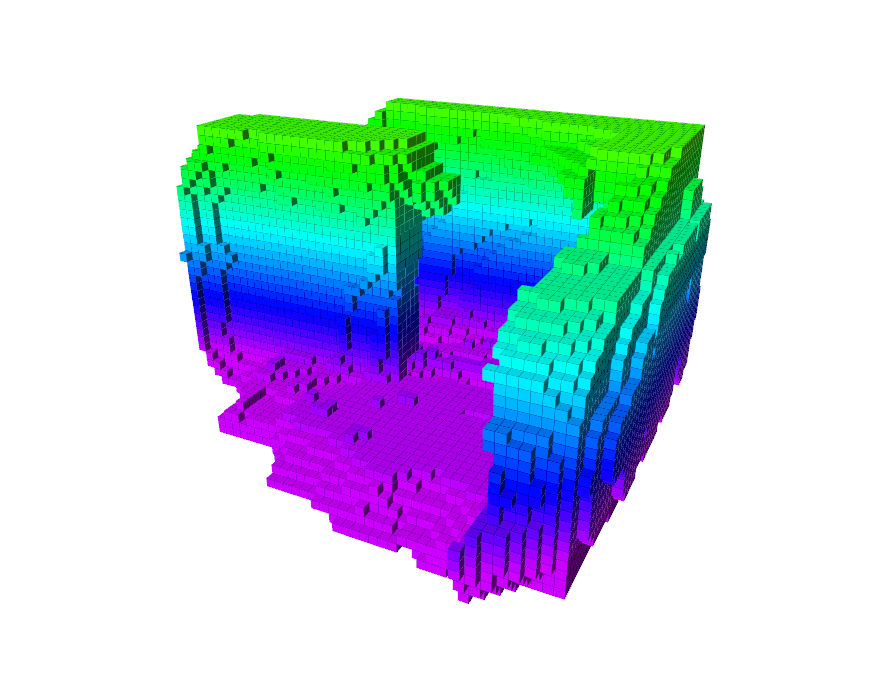
\includegraphics[width=0.23\linewidth]{img/long_term_gpoctomap_30}
	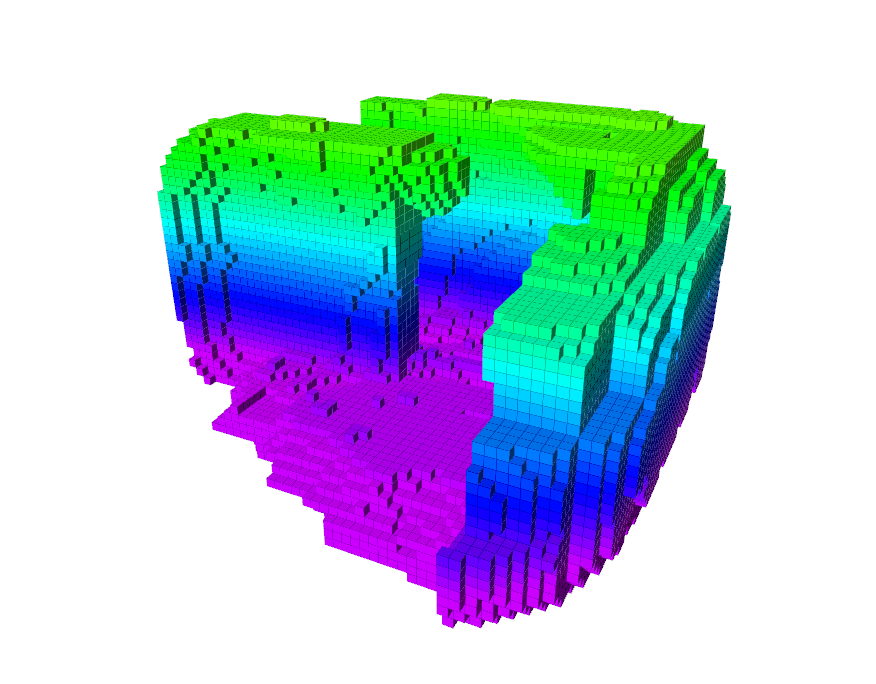
\includegraphics[width=0.23\linewidth]{img/long_term_gpoctomap_60}
}

\columnbreak

In this experiment, we simulate a robot keeping station, repeatedly scanning the same area. 

\textbf{Top}: Our method, BGKOctoMap updated with information from 1, 15, 30, and 60 scans (\textbf{left} to \textbf{right}) containing the same data.

\textbf{Bottom}: The result after applying the online Gaussian process occupancy mapping method in \cite{jwang} to the same data.

Qualitatively, our method (\textbf{top}) is more stable for long-term mapping scenarios with many repeat observations than the previous method (\textbf{bottom}) in which the occupied voxels tend to grow continuously with repeat observations.

\end{multicols}

\setlength{\columnsep}{0.1em}
\vspace{0.1em}
\begin{multicols}{2}

We quantitatively evaluated the inference model in both simulated environments. On the \textbf{left} we show the receiver operating characteristic (ROC) curve of the classifier for the \textit{structured} map, and for the \textit{unstructured} map on the \textbf{right}. Each point on the curve shows the false-positive rate and true-positive rate at a particular threshold separating the positive class "occupied" and the negative class "unoccupied" (up and to the left is better). The area under the curve measures the overall accuracy of the classifier. We compare our method to GPOctomap-NBCM-P presented in \cite{jwang} and standard OctoMap.
\\


{
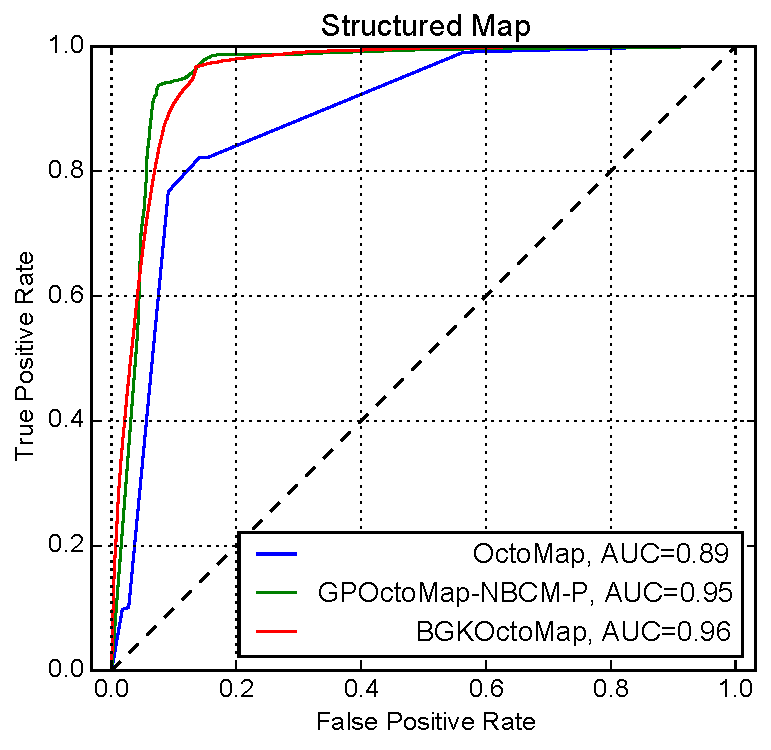
\includegraphics[width=0.468\linewidth]{img/sim_structured_roc}
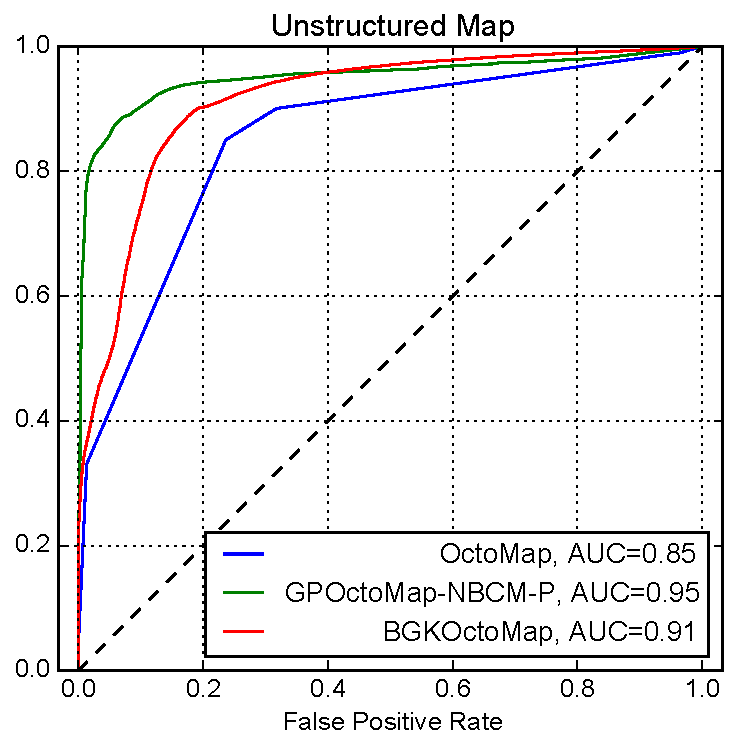
\includegraphics[width=0.45\linewidth]{img/sim_unstructured_roc} 
}

\end{multicols}

}


\end{poster}

\end{document}

